%# -*- coding: utf-8-unix -*-
%%==================================================
%% chapter01.tex for SJTU Master Thesis
%%==================================================

%\bibliographystyle{sjtu2}%[此处用于每章都生产参考文献]

\chapter{绪论}
\label{chap:introduction}

\section{大数据发展概述}
\label{sec:big data general}

计算机信息处理和存储技术的高速发展和快速普及,使得各个应用行业和科研领域的工作规模在数据上呈现爆炸式的增长。早期人们从数据规模出发用大数据(\emph{Big Data})对这一概念进行定义,现在大数据这一定义更多地从信息处理技术和需求方法出来,代表着我们从大数据分析与应用中所需求的新的应用和新的发展。随着计算机飞速进步的处理能力,我们能够从大数据挖掘中获取到我们所需要的应用价值。

大数据的定义以类型多、容量大、存取快、价值高为主的数据集合。现在世界上运用大数据推动经济发展、提升政府服务和提高用户生活体验正在成为一种主流的趋势,发达国家和发展中国家都在制定着与本国发展相符的大数据战略性文件以推动大数据在各个领域的发展和应用。目前,我国互联网和移动互联网的用户数目庞大,拥有丰富且系统的饿数据资源储备与广大应用市场优势。坚持大数据的驱动发展和部署范围,并拓展深化大数据的实际应用,已经成为稳增长、调结构、促改革、惠民生和推动政府治理能力现代化的内在需要和必然选择。

在大众创业和万众穿行的创新驱动新格局,充分利用已有的大数据红利并促进激发大众创业的活力是目前利用大数据发展的总体目标。政府在这一方面也鼓励从业与各个行业的人员利用已有开放共享的大数据资源,进行资源整合与分类,提升大数据的治理能力。在这一基础上推动相关产业一起创新发展,利用类型不同、数量众多的大数据资源来培育出新兴的产业领域,助力我国在目前阶段的经济转型。与此同时,大数据安全发展也需要得以保障,在开发大数据应用的时候提高管理水平和保证良性发展是我们再开发应用过程中所注意的方面。

\section{轨迹数据处理现有工作的概述及评价}
\label{sec:background}

传统企业数据、机器与传感器数据和社交数据被认为是如今大数据大致的三个类别。轨迹大数据主要属于机器与传感器数据。现代社会地理位置获取和移动计算科技进步,促使轨迹数据的大规模发展。这些轨迹数据体现了例如人类,车辆以及动物等移动物体的移动多样性。在过去十几年间,许多旨在处理、管理和挖掘轨迹数据的算法与技术许多应用中有着广泛而重要的应用价值。如今以轨迹数据挖掘为首的轨迹数据处理技术已经日趋系统且规范,从轨迹数据生成,到轨迹数据预处理,再到轨迹数据管理,最后到多样的数据挖掘任务(例如轨迹模式挖掘、轨迹异常检测、轨迹分类等等)。已有轨迹处理和轨迹挖掘的技术在相互应用中有着重要的联系与关联,轨迹数据转化成其他轨迹形式,例如图、矩阵和张量的方法也在越来越多的轨迹数据挖掘和机器学习领域有着常见的应用。

轨迹从概念上定义是一个移动物体的移动轨迹,轨迹数据可以用于许多领域的复杂分析。例如,公共交通系统可以应用过去时刻的轨迹数据分析交通流量模式并找出致使交通拥塞的原因;生物领域的动物长途迁移轨迹或是短途移动变化可以为人类提供宝贵的数据分析人类活动对生态环境的影响程度;还可以通过分析数据预测城乡车辆移动情况并及时提供符合公众出行的公共交通支持。其他应用领域也包括了路径优化设计,公共交通安全管理和基于兴趣点的用户个性化服务。

基于以上应用情景,轨迹数据挖掘在计算机科学、社会学和地理学领域都变得愈发重要。在轨技数据挖掘领域研究从深度和广度都已经取得了不错的成果,从图\ref{fig:1-1}\cite{zheng2015trajectory}可以看出当前轨迹数据挖掘与处理的基本研究步骤。本课题相似轨迹查询方法设计与实现主要基于其该范例中的轨迹预处理与轨迹数据索引与获取这两个领域中已存在的方法,并结合自己的理解和数据的格式实现改善和创新。

\begin{figure}[!htp]
  \centering
  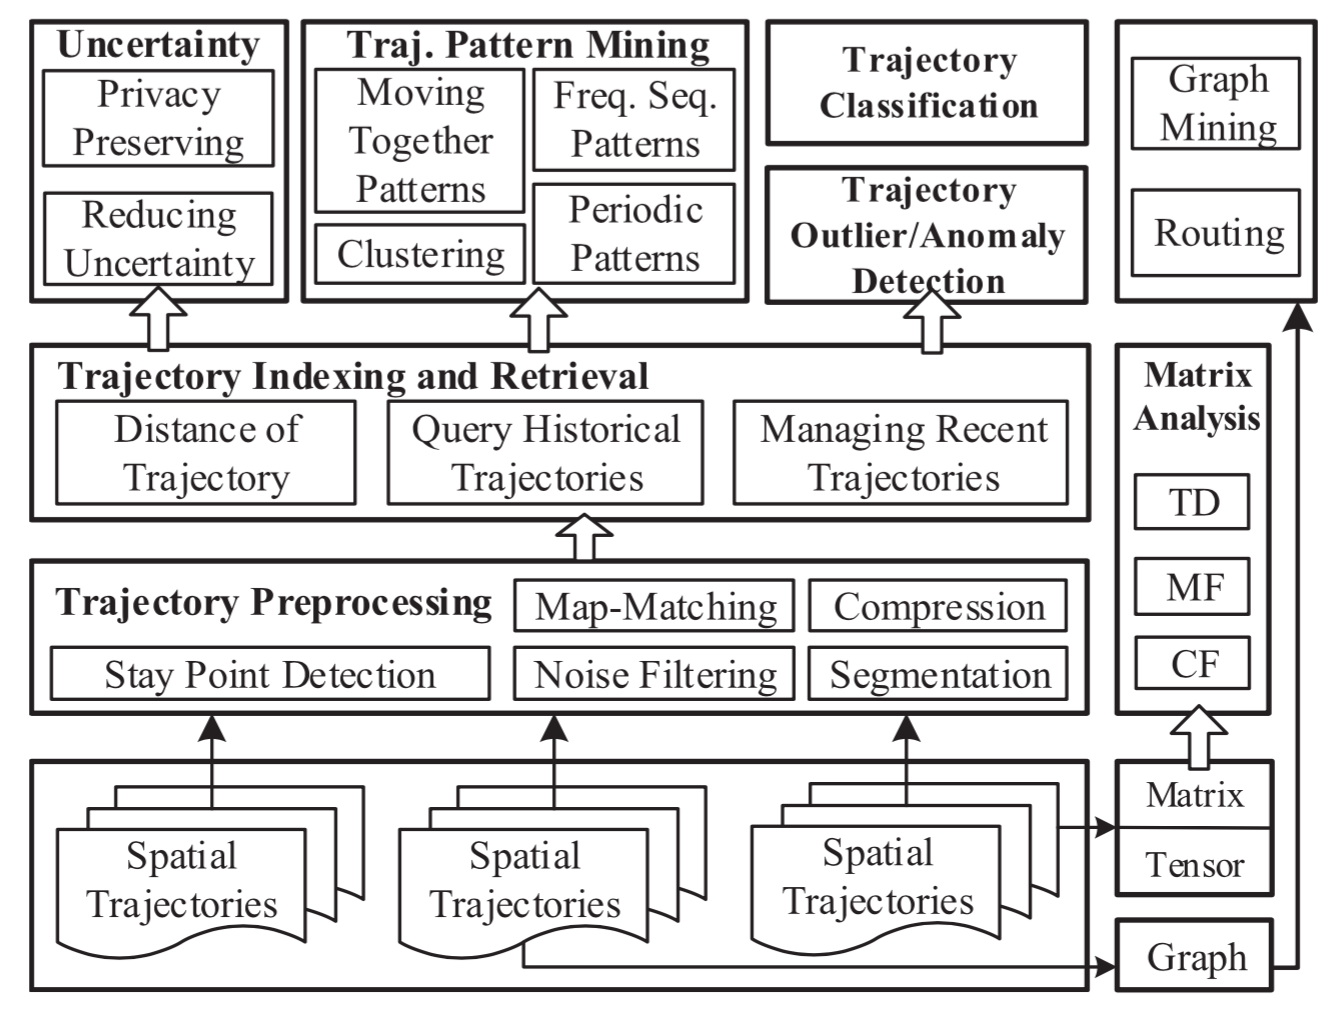
\includegraphics[width=0.7\textwidth]{chapter01/paradigm.png}
  \bicaption[fig:1-1]{轨技数据挖掘范例}{轨技数据挖掘范例}{Fig}{Paradigm of trajectory data mining}
\end{figure}

大量空间轨迹数据为我们提供了分析移动物体移动方式的可能性,这种移动方式的分析可以体现出单个轨迹所包含的某种特定移动方式或是一组轨迹所共享的相似移动方式。通常情况下相似轨迹查询是基于时空关系的查询,除此之外有些情况下一些相似轨迹查询会增加特定的查询条件,例如最快速度、偏移方向或是在规定的时间段内经过特定地理区域等等条件。在相似轨迹查询中缺少时间维度参数(时间戳或是时间段)是可以接受的,加入时间参数的相似轨迹查询本文将他们视为其中的一种特殊情况处理。
\\

\subsection{轨迹查询简介}
\label{sec:requirements}
完成在轨迹数据库中复杂的轨迹查询操作是复杂且费时的操作,因为轨迹数据库的规模一般是非常庞大的。因此,轨迹数据库的一个重要点事支持高效的轨迹索引以加速轨迹插叙过程。通常情况下,时空数据的索引技术是空间数据索引辅以时间度量参数。轨迹查询\cite{zheng2011computing}既关注经过的地理位置的拓扑位置顺序,也关注空间物体之间的距离度量,从简单的欧式距离度量到复杂的轨迹之间相似性。从大体上说,如今的轨迹查询依照时空关系分为三类:1)$P$-$query$,查询满足特定轨迹段或者时空关系的兴趣点或者查询针对某些兴趣点满足时空关系的轨迹;2)$R$-$query$,根据给定的时空区域查询轨迹或者给定轨迹查询目的区域,3)$T$-$query$, 查询在一组轨迹数据集中查询相似轨迹或在给定的距离阈值内查询轨迹。

\subsection{相似轨迹查询应用现状}
\label{subsec:searching trajectories application now}
相似轨迹查询主要是基于上述的轨迹查询方法中$P$-$query$和$T$-$query$展开的。

$P$-$query$主要应用在给定地理位置点后找到满足时空关系的轨迹或者轨迹段。单点轨迹查询找到针对某一给定地理位置点的最近轨迹。多点轨迹查询在给定一组地理位置点集后在轨迹数据里中找到能在地理位置意义上连接查询点集的多条轨迹。前者用以找到某一地理位置范围内的潜在轨迹。后者在制定行进轨迹路线中有着很好的应用。$T$-$query$通常通过聚类或分类轨迹在轨迹数据库中查询轨迹。轨迹分类和聚类算法在许多应用中有着广泛的应用,例如基于移动物体特征的轨迹测或是分析路网流量结构,在轨迹集合发现共同的子轨迹以及查询与目标轨迹在欧式距离上最接近的轨迹集合。

基于$P$-$query$的查询主要是衡量点到轨迹的中最近点的距离。目前也常通过拓展这一思路当多点的$P$-$query$查询以评价一条轨迹连接多个查询点的好坏。在$T$-$query$这一查询类型方面则有很多较为成熟的方法主要的不同在于他们各自的相似距离函数的定义,例如动态时间规划轨迹方法(Dynamic Time Warping)、最长公共子序列方法(Longest Common Subsequence)、基于编辑代价的方法(Edit Distance With Real Penalty)和基于序列编辑距离的方法(Edit Distance on Real Sequences)等等。这些方法在初期主要应用于时序相关的数据上,但是由于轨迹在某种意义上可以看成是多维度上的时序数据,上述的相似距离方法则可以应用上轨迹数据上。

\subsection{相似轨迹查询技术现状概述}
\label{subsec:searching trajectories technique now}
相似轨迹查询技术目前主要通过轨迹分类、轨迹聚类或计算轨迹距离度量这三种大概方法来实现。在这三类方法的实现中,对于相似轨迹之前匹配的模型建立和算法改进和对长度较长数据的分段算法是问题解决中的主要关注点。

\section{相似轨迹查询问题描述}
\label{sec:requirements}
\subsection{问题大致描述}
\label{subsec:question}
随着轨迹数据大规模的发展与存储,在日常生活中,如何高效查询轨迹对于用户或是在工业领域都有着重要的意义。特定情况下,查询类型也会根据需求有着变化。相似轨迹查询属于轨迹查询中的一种。在这里我们队相似轨迹查询问题进行大致描述;给定一组表示一条轨迹的轨迹数据点$Q$和轨迹数据库$D$,查询出在地理形状上与这些轨迹点所描述的轨迹的k条最相近的轨迹。

\subsection{相似轨迹查询方法设计概述}
\label{subsec:requirements}
本文研究的相似轨迹查询方法主要基于位置定的查询,即查询主要是基于一组有序或是无序的地理位置点。查询的首相要目标是从轨迹数据库中找出连接查询位置点的k条最佳连接轨迹(K Best-Connected Trajectories)使得这k条轨迹能够在地理位置上连接给定的未指定。不同于传统形状或其他查询标准通过给定一条轨迹的相似轨迹查询,本文的相似轨迹查询主要针对于所查找到的轨迹对于给定的一组轨迹点连接性的优劣。

如图\ref{fig:1-2}\cite{chen2010searching}所示,通过点击地图或图像地理解码给定一组地理位置点(图中点注释),我们可以从数据库中获取找一条能够连接给点地理位置点原始轨迹(图中线注释),该实例体现出本相似轨迹查询方法在能够在包括旅游路线规划等新兴应用中更好地服务用户。与此同时,这种相似轨迹查询能还能在以上场景有所应用:旅行社或自由行游客对出行经典的路径规划;动物园能调查出动物对到某些特定地点的最短路径;交通运输部门对本地市民城乡情况的规划。

\begin{figure}[!htp]
  \centering
  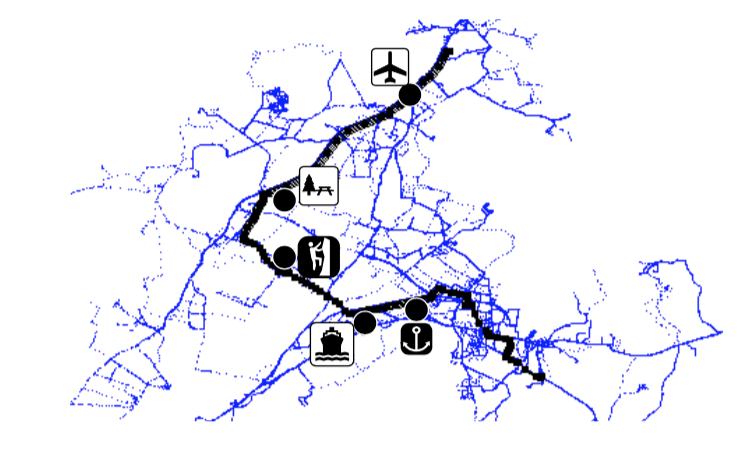
\includegraphics[width=0.5\textwidth]{chapter01/search-example.png}
  \bicaption[fig:1-2]{基于位置点的相似轨迹查询}{基于位置点的相似轨迹查询\cite{chen2010searching}}{Fig}{Similar trajectory search by locations}
\end{figure}

大体上,k条最佳连接轨迹查询基于的地理位置点需要具备必要的经纬度信息$(latitude,longitude)$。这些经纬度位置地点可以是旅游景点,不明确的沙滩或是任何一处地理坐标。用户可以通过决定轨迹连接有序或是无序以决定查询结果。例如一个简单的查询包括三个地理位置点 $A$,$B$,$C$

\begin{displaymath}
	{A_{(37.2601, 122.0941)}, B_{(37.2721, 122.0648)}, C_{(37.3344,122.1538)}}
\end{displaymath}

其中(37.2601, 122.0941)代表A点的经纬度地理坐标。如果查询附带有序条件,则查询轨迹结果应保留轨迹点之间的相对顺序性,即$A \rightarrow B \rightarrow C$。传统的相似轨迹查询方法显然无法解决查询结果与查询条件之间有序一致性。另外,本文所提出的轨迹查询方法基于任意的地理位置点使得查询模式更加多样和灵活。从本质上而言,这种这种查询方法的设计基于传统的单点查询方法以寻找针对某一位置的最为临近轨迹。

为了实现这一相似轨迹查询方法,本文首先对一组给定地理位置点中的每一个点进行基于点的查询以从数据库中找到最近的轨迹点。如果查询结果存在,通过对每一个结果的汇总所得出的轨迹从理论上而言是最接近查询点的一条轨迹且对给定的地理位置点具有良好的连接性。从这个思路出发,本文拓展K最近邻(k-NearestNeighbor algorithm)算法并提出增长性K最近邻($Incremental$ $k$-$NN$ $algorithm$)算法。该算法增长性获取每个查询位置点的最近轨迹并不断检查以查询到的轨迹。通过自定义的轨迹相似性上界与下界,借鉴备选和筛选的算法设计思路(candidate-refinement)来进行优化与剪枝。利用R树(R-Tree)作为地理位置点的索引结构,算法实现过程中根据具体计算机情况和性能需求选择性使用最好优先搜索(best-first)方法或是深度优先搜索(depth-first)方法进行查询。

\section{相似轨迹查询应用价值}
\label{sec:application value}
相似轨迹查询系统在实际情景中具有广泛的应用价值。在路径规划应用方面上,相似轨迹查询从已记录的历史轨迹中,根据用户定义有序或无序的旅游景点顺序,给出k条大致符合出行路径的历史轨迹基于用户参考并选出用户自己偏好的出行路径;在轨迹推荐或拼车推荐方面上,由于限号或出行限制问题,可以通过在历史轨迹中查询相似的轨迹查询出是否有在上下班或平时出行模式较为相似的多名用户,选择在有出行限制的时段与别的用户共享出行设备;在交通分析方面,相似轨迹查询可以为公安行业根据几个具体的地理位置点锁定一辆具有车载GPS设备的车辆。除此之外,相似轨迹查询的具体应用还有许多,不予以赘述。

\section{困难和挑战}
\label{sec:difficulty}
相似轨迹查询方法的设计与实现存在的以下主要的困难和挑战:1)高效准确实现相似轨迹查询。由于轨迹数据集的规模较大,通过常规查询和搜索会耗用大量时间和空间,而且在搜索过程中还要避免一些错误数据的加入。2)基于分布式的相似轨迹查询。相似轨迹查询领域的已有工作较为丰富,但是在单机层面上的查询处理。对于轨迹大数据处理而言,将相似轨迹查询移植与分布式环境操作是必要过程。3)实现基于相似轨迹查询功能的软件系统。轨迹数据处理的价值在于通过轨迹数据处理为每个客户提供特定服务。在相似轨迹查询中,需要提供一个用户界面为用户查询相似轨迹并将轨迹可视化的软件系统,在满足高效查询过程中需要保证良好的软件系统交互性。

\section{论文结构}
\label{sec:requirements}
毕业设计论文主要结构为:本章绪论介绍轨迹数据处理和相似轨迹查询的相关背景,以及在该背景下对相似轨迹查询这一问题的概要描述,在该问题下所面临处理困难和挑战;第二章以相关工作为主,介绍本文相似轨迹处理查询方法设计与实现所设计到的相关理论算法基础和有关设计技术支持;第三章从实现算法入手,介绍具体的实现细节和分布式实现方法;本文第四章和第五章分别介绍开发相似轨迹查询系统的需求分析和设计概要,前者作为设计指导,明确本文应该从什么方向针对性地去进行系统设计;第六章作为系统测试和评价章节;最后对本文所涉及的工作进行总结和未来展望。

\section{本章小结}
\label{sec:requirements}
本章节已经初步介绍了相似轨迹查询这一概念和其相关背景,由于目前的在轨迹数据处理已经系统和规范的处理流程,轨迹数据挖掘这一领域的方法技术也已经较为成熟且丰富,通过学习传统的相似轨迹查询方法和他们各自的应用经验,本文所提出的方法在已有成果的基础上进行进一步的创新与优化,便可以使得相似轨迹查询方法与传统的相似轨迹查询有着较大的不同,且具有特定查询环境上的查询优势与性能优化。在对相似轨迹查询问题进行大致描述后,本文对解决这一问题在现实生活中有哪些具体的应用进行展开,并初步描述解决相似轨迹查询这一问题所产生的实际价值。

解决相似轨迹查询这一问题的过程中也伴随着一些具体的困难与挑战。本文通过拓展如今最为基本的k最近邻数据挖掘技术,以实现基础的相似轨迹查询方法为基本理论目的,移植单机运行代码至分布式环境系统为应用目标,开展毕业设计课题。


